

\chapter{Product evaluation and AI assistant in VitamiNurse}
\section*{Introduction}
\addcontentsline{toc}{section}{Introduction}
The VitamiNurse app stands out from other traditional nutrition apps through its advanced use of artificial intelligence .

In addition to the use of a sentence transformer model to generate vector embeddings in the recommendation system discussed earlier, this section introduces two key AI components: a product evaluation system and an AI assistant.

This integration of AI transforms static product recommendations into an interactive dialogue system that is available 24/7 to answer questions and provide nutritional guidance. The following sections detail the architecture and functionality of these AI systems within the VitamiNurse mobile app.

\section{Advanced scan system with AI analysis }

Instead of showing large amounts of raw product data, it uses AI to interpret the product after scanning its barcode.  Through the combination of detailed nutritional information, user health profiles, and AI reasoning based on prompts, the VitamiNurse app provides customized nutritional guidance in a way that traditional tools cannot. The result is a highly interactive and user-friendly experience that transforms a simple scan into an informed decision-making process.

\subsection{Prompt Engineering for AI Analysis}
\par In addition to the details of the product that appear on the screen after scanning the barcode, we added an AI analytics system to provide a concise and personalized conclusion.
 The generative AI capabilities of our system are powered by a popular pre-trained LLM, which is ChatGPT-4, to build accurate and relevant responses.
 \par The system uses structured prompts to guide AI during product evaluation.
The following code illustrates how each prompt integrates essential product information with user-specific data, including health conditions and allergies, to determine the suitability of the product for the user profile.
 \begin{center}
    \begin{figure}[H]
    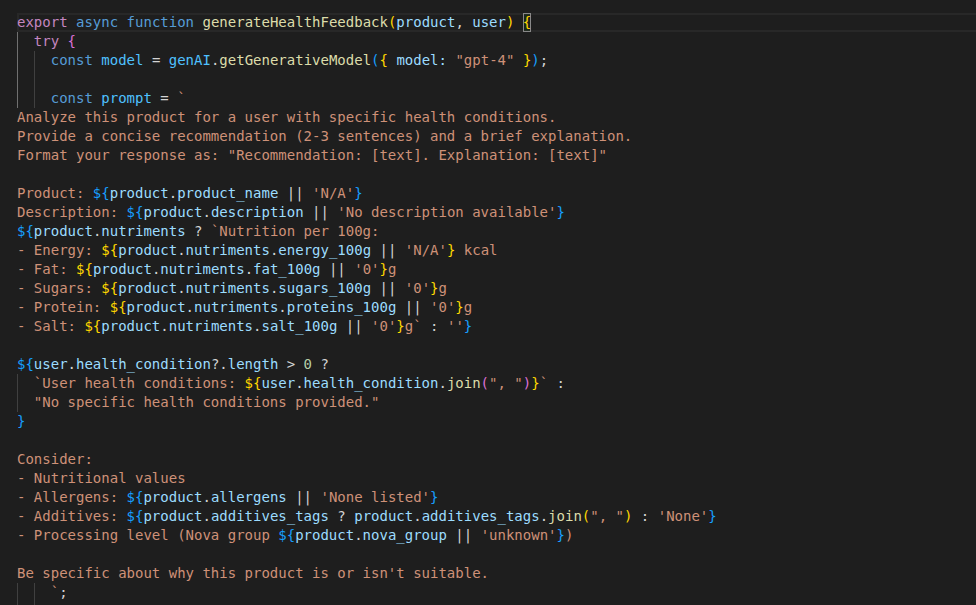
\includegraphics[width=0.9\textwidth]{images/prompt_engineering.png}
    \caption{Prompt Engineering Using GPT-4} 
    \label{fig:Prompt Engineering}
\end{figure}
\end{center}

\subsection{System operation in VitamiNurse}
The AI analysis system in VitamiNurse integrates a product scanning feature with real-time health feedback, powered by a combination of external APIs, a MongoDB database, and the ChatGPT-4 model. Users can scan a barcode (EAN) to retrieve detailed nutritional information, which is cross-referenced with their health profile stored in the users collection. The system first checks our database for existing product data. If it is unavailable, it fetches data from the OpenFoodFacts API and caches it for future use. The AI then processes these data alongside user health conditions to generate personalized feedback: \textbf{Is this product suitable or not, and why?}
The following picture illustrates how the user see the details of the scanned product and generated health feedback by the AI analytics system:

\begin{figure}[h!]
    \centering
    % First image
    \begin{subfigure}[b]{0.23\textwidth}
        \centering
        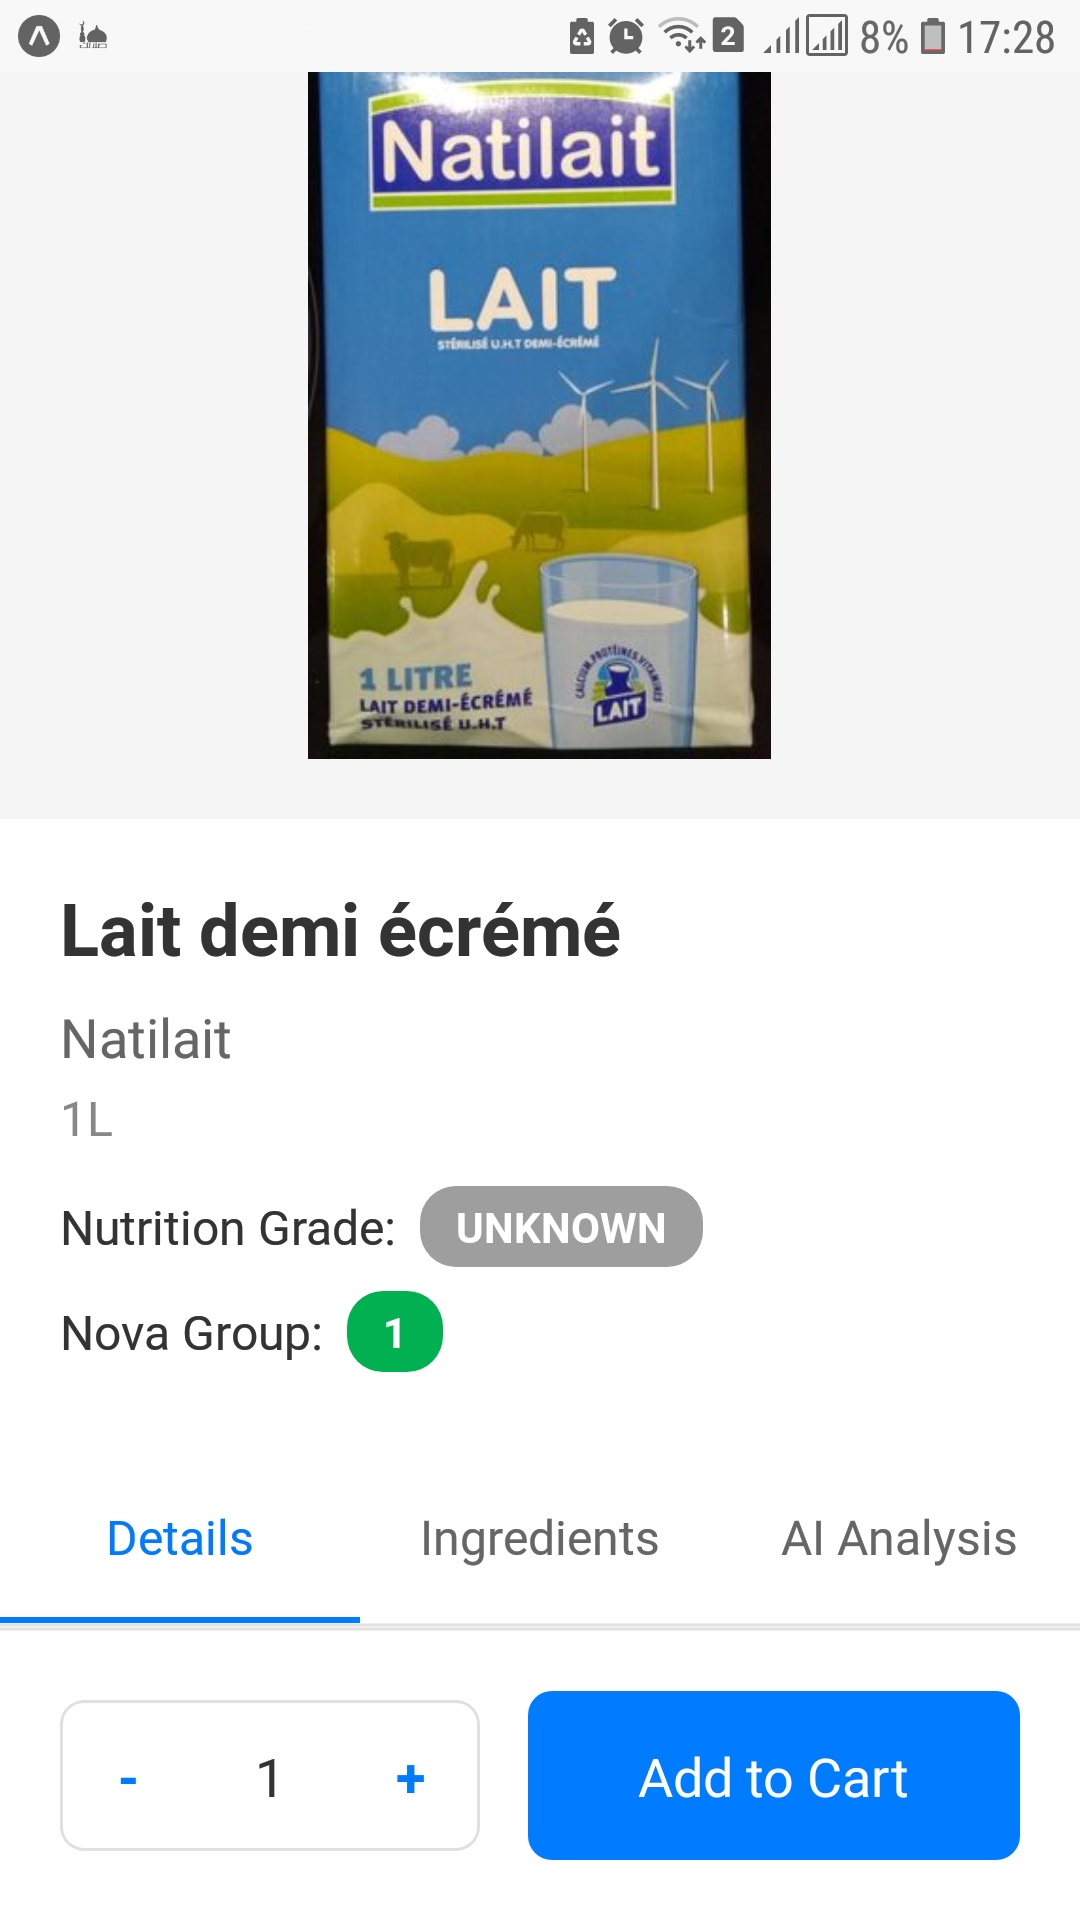
\includegraphics[width=\textwidth]{images/natilait1.jpg}
    \end{subfigure}
    % Second image
    \begin{subfigure}[b]{0.23\textwidth}
        \centering
        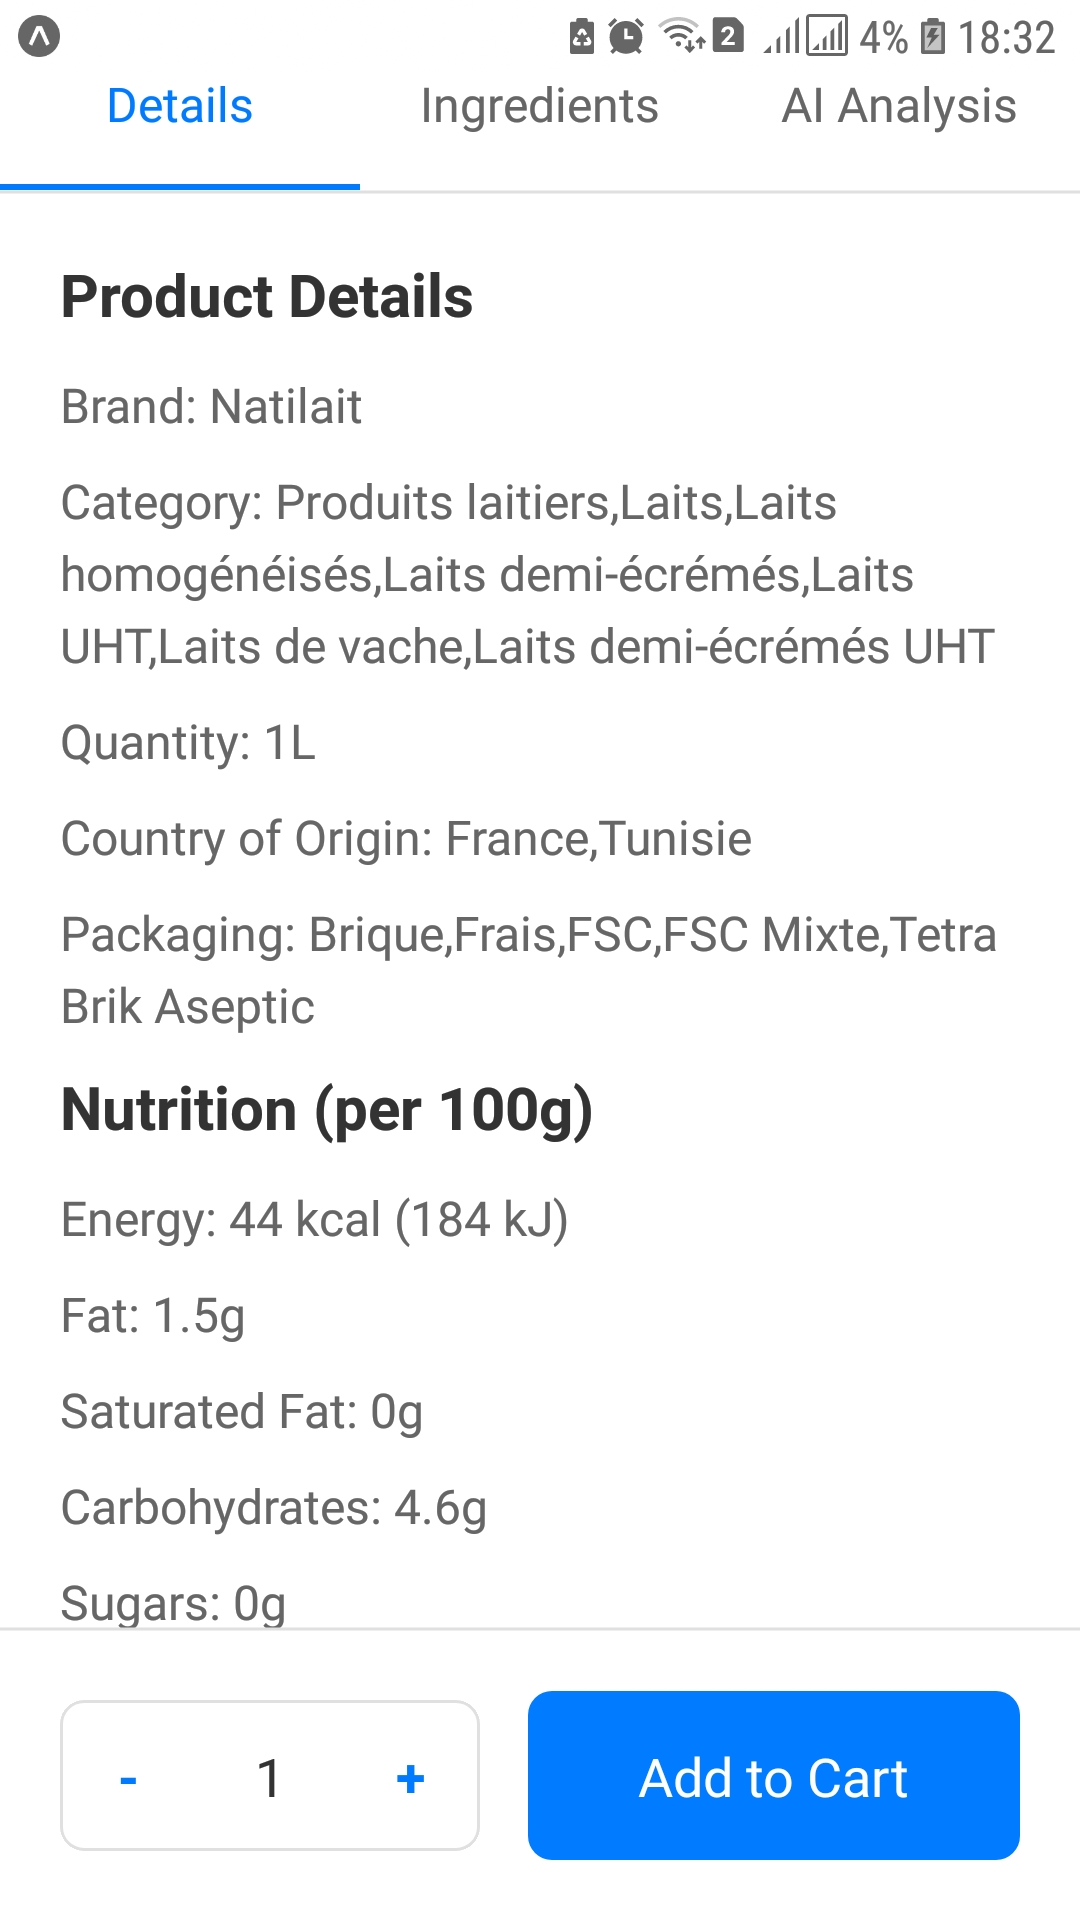
\includegraphics[width=\textwidth]{images/natilait2.jpg}
    \end{subfigure}
    % Third image
    \begin{subfigure}[b]{0.23\textwidth}
        \centering
        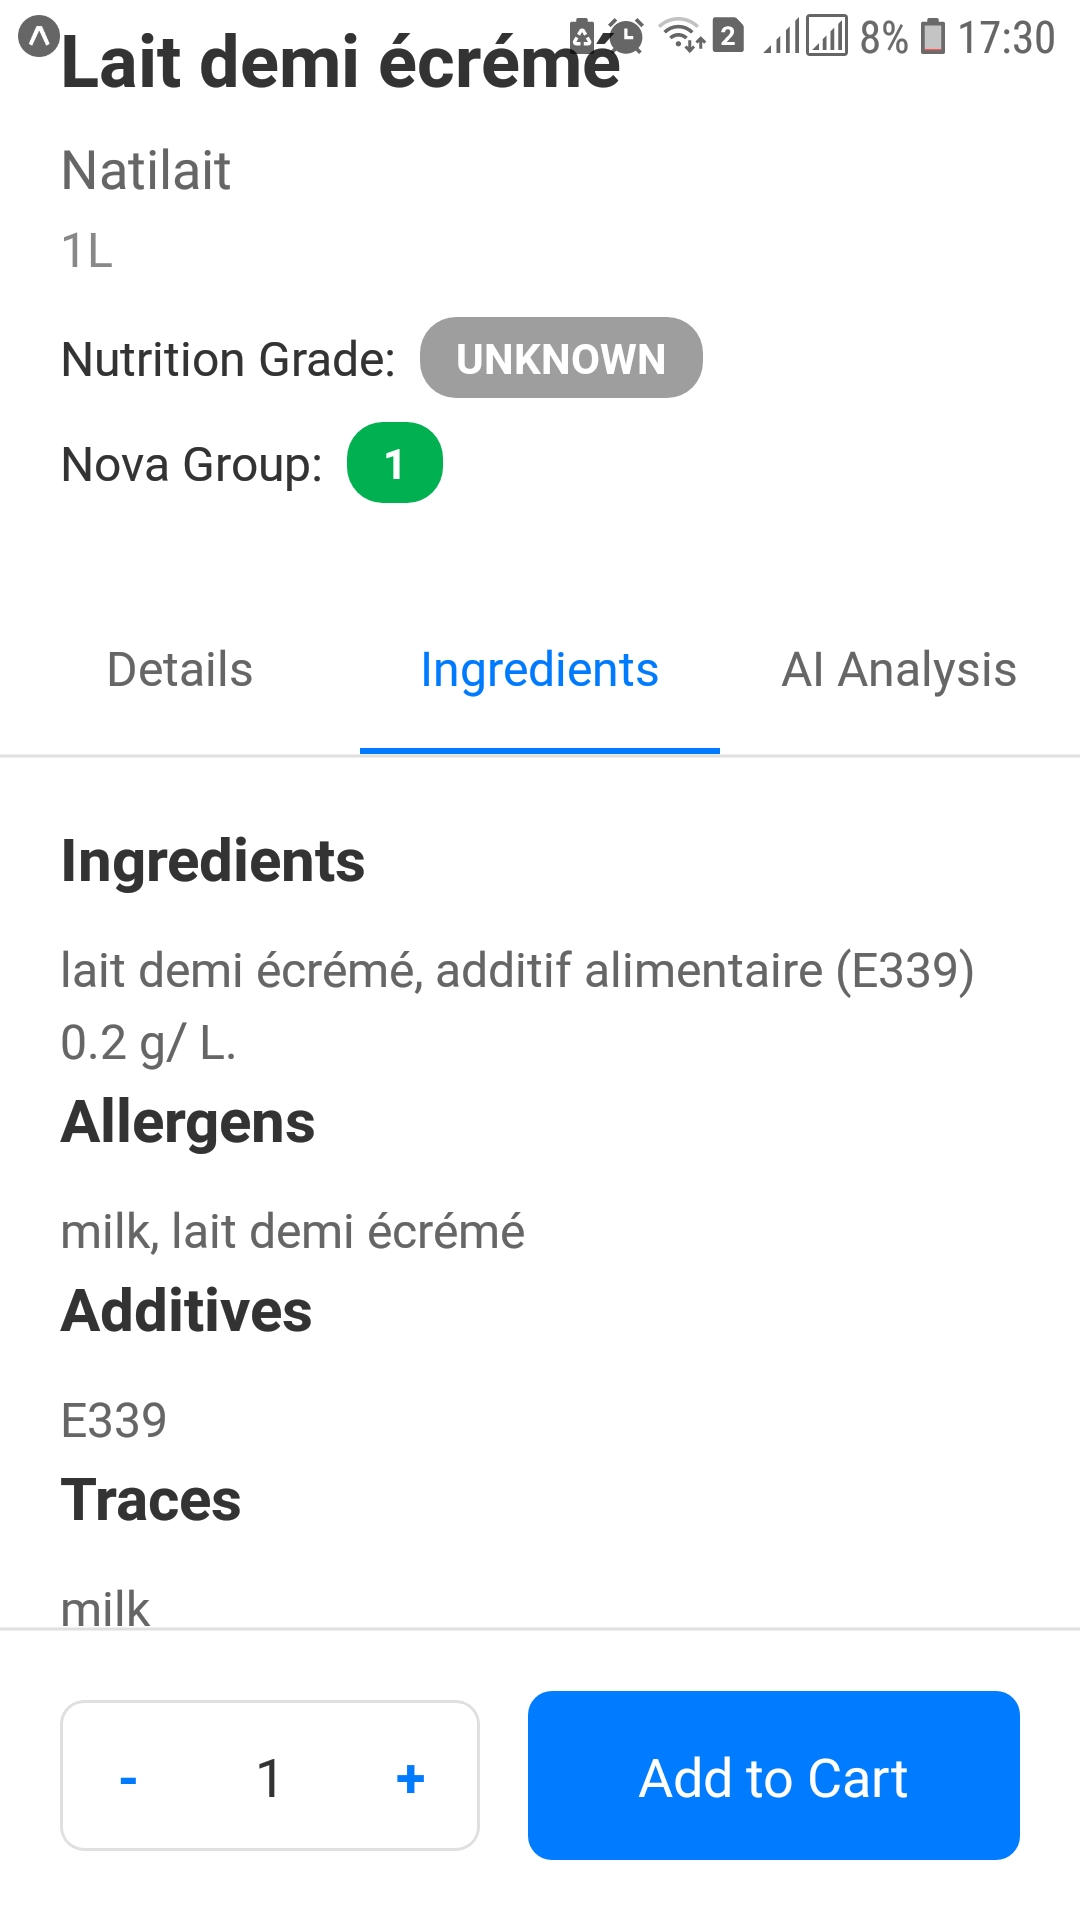
\includegraphics[width=\textwidth]{images/natilait3.jpg}
    \end{subfigure}
    % Fourth image
    \begin{subfigure}[b]{0.23\textwidth}
        \centering
        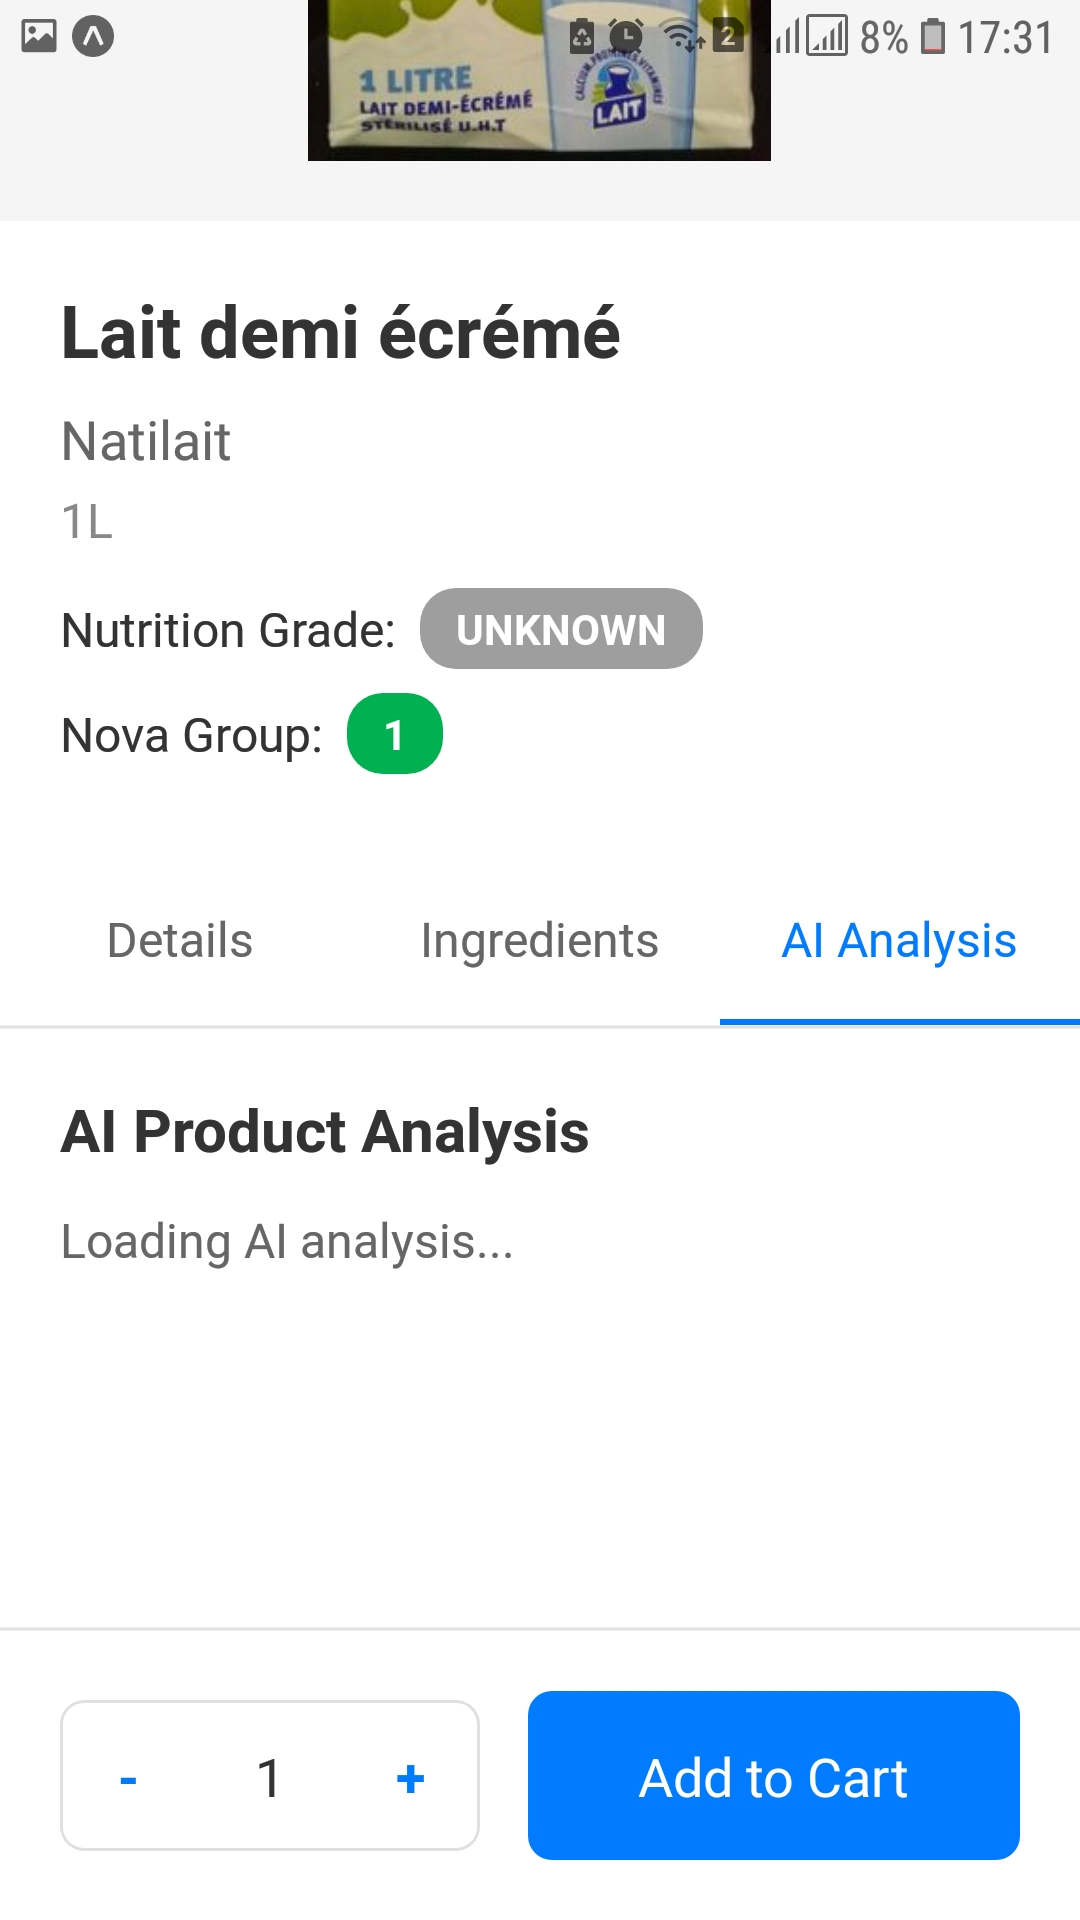
\includegraphics[width=\textwidth]{images/natilait4.jpg}
    \end{subfigure}
\end{figure}


\section{The AI Assistant}
The AI nutrition assistant represents a new generation of personalized dietary advice and nutritional data analysis, all within a coherent conversational interface.
\section{System Architecture}
The architecture of the Nutrition Assistant is designed for modularity, scalability, and maintainability. Figure~\ref{fig:chatbot Architect} outlines this three-tier architecture, consisting of the user mobile interface, backend server, and AI/data layer.
 This separation ensures that improvements in one layer, such as up-
grading the recommendation logic, can be implemented without disrupting other components of the system. The conversational capabilities of this intuitive chatbot are tightly integrated with a persistent memory framework in order to recall previous user interactions and adapt recommendations over time.  
 \begin{center}
    \begin{figure}[H]
    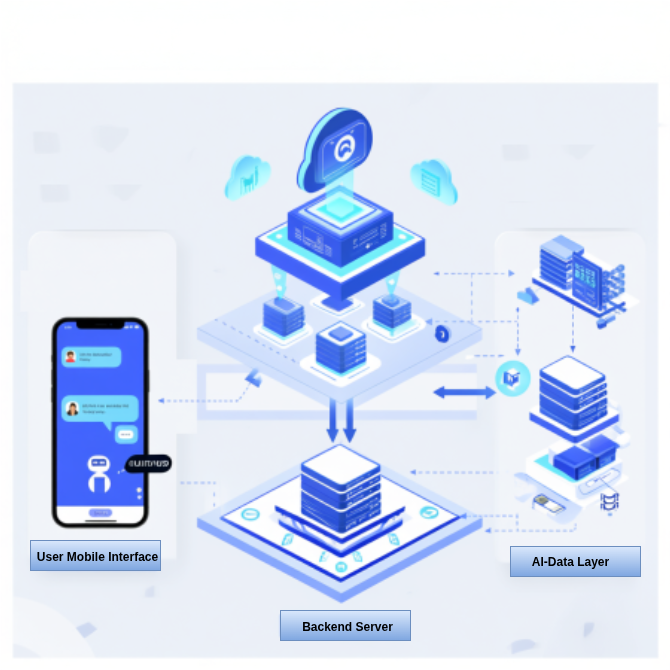
\includegraphics[width=0.9\textwidth]{images/chat_layers.png}
    \caption{Chatbot Architecture} 
    \label{fig:chatbot Architect}
\end{figure}
\end{center}

\subsection{User Mobile Interface}
The mobile interface serves as the primary point of interaction between the user and the VitamiNurse assistant. It supports both chat bubble and product scans. When a user scans a product barcode or types a question, the interface sends a structured request to the backend, which in turn invokes the AI modules for analysis. The design emphasizes simplicity and readability, ensuring that even complex nutritional assessments are communicated in concise, easy-to-understand language. This is achieved through the adoption of a fixed “Recommendation + Explanation” format, which the AI adheres to when generating responses. The application return the scanned products details and nutritional breakdowns as well as AI analysis for this product, making the experience both informative and engaging.

\subsection{Backend (FastAPI Server)}
The backend, developed using the \texttt{FastAPI} framework, functions as the system’s control hub. It is responsible for orchestrating communication between the mobile interface, AI reasoning layer, and data storage modules. Upon receiving a request, the backend validates the input, retrieves relevant product data from the nutritional database, and enriches it with user-specific profile information. It then constructs a prompt to be sent to the large language model (LLM), ensuring that all relevant dietary constraints and health conditions are explicitly included. The backend also maintains user session management, conversation history storage, and security protocols for handling sensitive health-related information. Thanks to FastAPI’s asynchronous capabilities, the backend can handle concurrent user requests with minimal latency, which is crucial for providing real-time responses.
 \begin{center}
    \begin{figure}[H]
    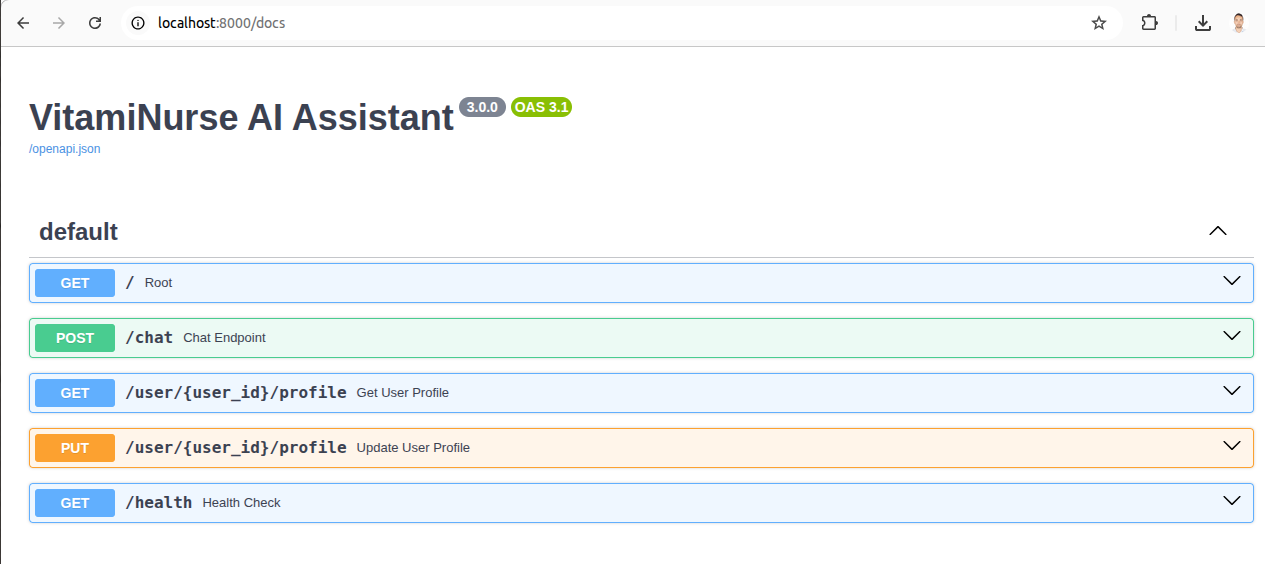
\includegraphics[width=0.9\textwidth]{images/chatbot_API.png}
    \caption{Chatbot FastAPI} 
    \label{fig:chatbot API}
\end{figure}
\end{center}

\subsection{AI and Data Layer}
The AI and data layer forms the intelligent core of the VitamiNurse assistant, leveraging advanced language models and sophisticated intent detection to deliver personalized nutritional guidance. At the heart of the system is OpenAI's \texttt{gpt-4o-mini} model, which is meticulously engineered through prompt crafting to provide structured, scientifically-grounded nutritional advice.

The system employs \texttt{LangChain} as its orchestration framework, enabling sophisticated intent detection and parallel processing of user requests. Through LangChain's structured output parsing with Pydantic models, the assistant can simultaneously handle multiple user intents including product searches, recipe generation, profile updates, and general nutritional inquiries.

A \texttt{ChromaDB} vector database serves as the persistent storage layer, maintaining semantic embeddings of user profiles, conversation history, and product information. This enables efficient retrieval and contextual understanding while ensuring data persistence across sessions.

The \emph{Recommendation Engine} introduced in the previous chapter is seamlessly integrated into this architecture. It operates on a hybrid approach combining collaborative filtering and content-based filtering, ensuring that recommended products are both personalized and nutritionally appropriate for each user's specific profile and constraints.

\section{Key Features and Implementation}

\subsection{Parallel Intent Processing with LangChain}
A distinctive feature of the VitamiNurse assistant is its ability to process multiple user intents simultaneously using LangChain's parallel processing capabilities. The system employs specialized chains for:
\begin{itemize}
\item \textbf{Product Search}: Detecting product queries and EAN codes, searching ChromaDB, and invoking the recommendation API
\item \textbf{Recipe Generation}: Analyzing culinary preferences and generating personalized recipes using GPT-4
\item \textbf{Profile Management}: Extracting and updating user information from conversational context
\item \textbf{General Queries}: Handling nutritional questions and educational content
\end{itemize}

This parallel architecture ensures that users receive comprehensive responses addressing all aspects of their queries without sequential processing delays.

\subsection{Dynamic User Profile Intelligence}
The assistant's personalization engine is driven by an intelligently evolving user profile defined through Pydantic models. The system automatically extracts and updates profile information from natural conversations using GPT-4's extraction capabilities. Key profile attributes include:
\begin{itemize}
\item Dietary restrictions and allergies
\item Health conditions and medical considerations
\item Nutritional goals and preferences
\item Pregnancy status and special requirements
\item Favorite foods and taste preferences
\end{itemize}

The profile management system employs smart merging strategies that only update changed information while preserving existing valid data. This dynamic updating occurs in real-time during conversations, allowing the assistant to immediately incorporate new user information into its recommendations.

\subsection{AI-Powered Recipe Generation}
The system features an advanced recipe generation capability that creates personalized meal suggestions based on multiple factors:
\begin{itemize}
\item User's dietary restrictions and allergies
\item Detected cuisine preferences from conversation
\item Nutritional requirements and health goals
\ ingredient availability and preparation complexity
\end{itemize}

Recipes are generated entirely by GPT-4 and structured into standardized JSON format containing complete nutritional information, preparation steps, cooking times, and customization suggestions. This approach ensures recipes are both personalized and practical for everyday use.

\subsection{Integrated Recommendation System}
The recommendation engine works in concert with the conversational AI to provide context-aware product suggestions. The integration follows a sophisticated workflow:
\begin{enumerate}
\item Intent detection identifies product-related queries
\item ChromaDB performs semantic search for relevant products
\item The recommendation API processes user-specific constraints
\item Results are filtered based on dietary rules and nutritional quality
\item GPT-4 generates natural language explanations of recommendations
\end{enumerate}

This seamless integration ensures that product recommendations are not only relevant to the search query but also safe and appropriate for the user's specific health profile and nutritional needs.

The architecture represents a significant advancement in conversational AI for healthcare applications, demonstrating how LangChain can orchestrate complex multi-intent processing while maintaining coherent, personalized user experiences.

\section{Challenges and Solutions}
Throughout development, several significant challenges emerged in creating a robust conversational nutrition assistant. Maintaining coherent conversation context across extended interactions was addressed through LangChain's sophisticated memory management and ChromaDB's persistent conversation storage. Personalizing recommendations without burdening users with excessive input requirements was solved through GPT-4's intelligent information extraction capabilities, which automatically detect and update user profiles from natural conversation.

Ensuring structured, explainable nutritional advice was achieved through rigorous prompt engineering and Pydantic output parsing, enforcing consistent response formats. Handling ambiguous or incomplete user queries was resolved through the parallel intent processing architecture, which allows multiple interpretation paths to be explored simultaneously before synthesizing a comprehensive response.

The integration of multiple AI components (LangChain chains, GPT-4, ChromaDB, and the recommendation API) presented coordination challenges that were overcome through asynchronous processing patterns and robust error handling mechanisms.

\section{Future Improvements}
Planned enhancements focus on expanding the assistant's capabilities and integration points. Multi-modal support will enable image-based food recognition and nutritional analysis through advanced computer vision integration. Expanded wearable device connectivity will incorporate real-time physiological data from fitness trackers and health monitors, allowing for dynamic nutritional adjustments based on activity levels and metabolic states.

Advanced personalization through reinforcement learning will enable the system to continuously improve its recommendations based on user feedback and outcomes. Voice interaction capabilities will be enhanced through integration with popular voice assistants (Alexa, Google Assistant) and development of custom voice interfaces for hands-free nutritional guidance.

Additional planned features include:
\begin{itemize}
\item \textbf{Meal Planning Automation}: Multi-day meal planning with grocery list generation
\item \textbf{Social Features}: Community recipe sharing and nutritional challenges
\item \textbf{Healthcare Integration}: EHR connectivity for medical condition management
\item \textbf{Advanced Analytics}: Nutritional intake tracking and trend analysis
\end{itemize}

\section{Conclusion}
The VitamiNurse AI Nutrition Assistant represents a significant advancement in conversational healthcare applications by successfully integrating the Recommendation Engine into a sophisticated LangChain-powered architecture. The system demonstrates how parallel intent processing, dynamic profile management, and AI-generated content can create a comprehensive nutritional guidance platform.

By leveraging LangChain's orchestration capabilities alongside GPT-4's generative power and ChromaDB's persistent storage, VitamiNurse delivers personalized, context-aware dietary recommendations that adapt to users' evolving needs. The architecture successfully balances conversational flexibility with structured nutritional guidance, providing both immediate answers and long-term nutritional support.

This implementation positions VitamiNurse as a scalable foundation for digital health interventions, with the potential to expand into various healthcare domains beyond nutrition. The modular design ensures adaptability to new data sources, interaction modalities, and user requirements, making it well-suited for the evolving landscape of AI-powered healthcare applications.

The assistant not only provides immediate nutritional guidance but also serves as an educational tool, helping users develop sustainable healthy eating habits through personalized, explainable recommendations that consider their unique circumstances, preferences, and goals.

